\chapter{Stellar rotation period inference using Gaussian processes}
\label{chapter:GP}

\begin{abstract}
The light curves of spotted, rotating stars are often non-sinusoidal and
quasi-periodic---spots are not static on the stellar surface and have finite
lifetimes causing stellar flux variations to slowly shift in phase.
A strictly periodic sinusoid is therefore not a representative generative
model for the light curve of star with a rotational signal.
Ideally, a physical model of the stellar surface would be conditioned on the
data, however the parameters of such models can be highly degenerate
\citep[\eg][]{Russell1906, Jeffers2009}.
Instead, we use an appropriate {\it effective} model: a Gaussian Process (GP)
with a quasi-periodic covariance kernel function.
By modelling the covariance matrix of the light curve with a GP, a highly
flexible semi-parametric function, we avoid the necessity to choose a `best
fitting' functional form, whilst sampling directly from the posterior
probability distribution function of the periodic parameter and marginalising
over the other kernel hyperparameters.
We used \nlightcurves\ simulated light curves with a range of rotation periods
to test the GP model.
We attempted to recover the rotation periods using three methods: our GP
method, a sine-fitting periodogram method and an autocorrelation function
method.
The posterior probability distribution of the rotation period parameter was
sampled using the affine invariant ensemble MCMC sampler {\tt emcee}
\citep{Foreman-Mackey2013}, and the GP operations were performed using the
{\tt george} python package \citep{George}.
Rotation periods inferred via this method are more precise and accurate than
the periodogram and ACF methods.
Furthermore, the improvement is expected to be even more dramatic when applied
to real, noisy {\it Kepler} light curves, since the GP method is well suited
to modelling rotation signals and correlated noise simultaneously.

\end{abstract}

\section{Introduction}

The light curves of spotted, rotating stars are often non-sinusoidal and
Quasi-Periodic (QP).
These stars vary in brightness due to active regions on their surfaces which
rotate in and out of view.
The non-sinusoidal quality is caused by the complicated surface spot patterns
and the quasi-periodicity is produced both by the finite lifetimes of these
active regions and the presence of differential rotation on the stellar
surface.
A strictly periodic sinusoid is therefore not a good model for stellar light
curves.
In an ideal world, a physical model of the stellar surface would be
conditioned on the data.
A physically realistic, generative model would perfectly capture the complexity
of shapes within stellar light curves as well as the quasi-periodic nature,
allowing for extremely precise probabilistic period recovery.
However, such physical models require many free parameters in order to
accurately represent a stellar surface and some of these parameters are
extremely degenerate.
In addition to global stellar parameters such as inclination and rotation
period, each spot or active region should have (at minimum) a longitude,
latitude, size, temperature and lifetime.
Considering that many stars have on the order of hundreds of spots, the number
of free parameters quickly becomes unwieldy, especially if the posterior PDFs
of these parameters are explored with MCMC.
Simplified spot models, such as the one described in \citet{Lanza2014} where
only two spots are modelled, have produced successful results, however these
simplified models sacrifice some precision due to lack of model flexibility.
Instead of using a physical model for stellar light curves, we choose to use
an {\it effective} model: one which captures the behaviour but is not
physically motivated, although the parameters of this model may be {\it
interpreted} as physical ones.
An ideal effective model for the light curve of a spotted, rotating star is
one with a small number of non-degenerate parameters that is flexible enough
to perfectly capture non-sinusoidal, QP behaviour.
These requirements are perfectly fulfilled by a Gaussian process (GP) model.

The standard methods used for measuring rotation periods include detecting
peaks in a Lomb-Scargle \citep{Lomb1976, Scargle1982} (LS) periodogram
\citep[e.g.][]{Reinhold2013}, Auto-Correlation Functions (ACFs)
\citep{Mcquillan2013} and wavelet transforms \citep{Garcia2014}.
The precision of the LS periodogram and wavelet methods are limited by the
suitability of the model choice.
A sinusoid is used in the case of the LS periodogram and the wavelet method
relies on a choice of mother wavelet that is assumed to describe the data over
a range of transpositions \citep[see, \eg][]{Carter2010}.
In contrast, the ACF method is much better suited to signals that are
non-sinusoidal.
In fact, it doesn't matter what shape the signal is: as long as it is
approximately periodic the ACF will display peaks located at the rotation
period.
A drawback of the ACF method however, is that it requires data to be
evenly-spaced\footnote{\citet{Edelson1988} describe a method for computing
ACFs for unevenly-spaced data.} which is not the case with \Kepler\ light
curves (although in many cases it can be approximated as uniformly sampled).
An ACF is also an operation performed on the data, not a generative model of
the data and is therefore not inherently probabilistic.
For this reason it is very difficult to estimate the uncertainty on an ACF
rotation period measurement.
Many rotation periods in the literature have been inferred by measuring the
position of the first peak in an ACF, however this approach can be dangerous.
The exponential decay in correlation can shift the peak position short-wards
of its true value, leading to an underestimate of the period.
We return to this point in section \textsection \ref{sec:discussion}.
% In order to avoid this, a period should be inferred by modelling the entire
% ACF, not just measuring the position of the first peak.

The motivation for developing a GP-based method for rotation period inference
is, firstly to measure more accurate and precise rotation periods using a
better-suited generative model than a sinusoid for the reasons explained
above.
Secondly, in order to infer {\it probabilistic} periods, i.e. to estimate the
posterior PDF of the rotation period and thereby measure a realistic and
representative uncertainty.
And thirdly, to allow for an additional correlated noise model to be included
during regression, the parameters of which could be marginalised over.
% And fourthly to provide some way of determining whether a periodic model is
% supported by the data over a purely stochastic one.

GPs are commonly used in the machine learning community and increasingly
in other scientific fields, for example biology and geophysics (where GP
regression is called `kriging').
More recently, GPs have been used in the astronomy literature \citep[see
\eg][]{Gibson2012, Haywood2014, Haywood2015, Evans2015, Rajpaul2015,
Rajpaul2016, Aigrain2016}.
% FIXME: CITATIONS Gibson, Aigrain, Evans, Rajpaul, Waldman(?), Cosmology,
% geology, biology, Rasmussen & Williams, etc.
They are useful in regression problems involving any stochastic process,
specifically when the probability distribution for the process is a
multi-variate Gaussian.
If the probability of obtaining a data-set is a Gaussian in $N$ dimensions,
where $N$ is the number of data points, that data-set can be described as, and
with, a Gaussian process.
An in-depth introduction to Gaussian processes is provided by
\citet{Rasmussen2005}.

GP models parameterise the covariance between data points and a kernel
function provides the form of covariance matrix parameterisation.
For example, take the time-series in figure \ref{fig:GP_example}.
% This is a \kepler\ light curve of Earth-like planet host Kepler-452: a G-type
% star that rotates once every $\sim$ 15 days.
This is the \kepler\ light curve of KID 1430163, a relatively active star that
rotates once every $\sim$ 4 days.
The stochastic variability in this time-series is typical of \kepler\ FGK
stars.
Clearly, data points in this light curve are correlated.
Points that are close together in time are tightly correlated and those that
are far apart are loosely correlated.
It is the way in which the covariance varies with the separation between data
points that is modelled when using GP regression.
It is not the data but the {\it covariance structure} that is modelled.
This fact is what gives GPs their flexibility---they can model any time
series with a similar covariance structure.
In addition, a very simple function can usually capture the covariance
structure of a light curve, whereas a much more complicated one may be
required to model the time-series itself.
% The light curve of \Kepler-452 has been modelled with a GP in figure
% \ref{fig:GP_example}, shown in orange.
The light curve of this star has been modelled with two different GP kernel
functions in figure \ref{fig:GP_example}, shown in blue and pink.
Both provide adequate fits to the data, however only the periodic kernel
function, `QP' is a useful model because it has a periodic parameter.
I return to this point shortly.

A range of kernel functions could be used to describe stellar variability.
For example, the simplest and most commonly used kernel function, the `Squared
Exponential' (SE) produces an adequate fit to the KID 1430163 light curve.
The SE kernel function is defined as,
\begin{equation}
k_{i,j} = A \exp \left(-\frac{(x_i - x_j)^2}{2l^2} \right).
\end{equation}
\label{eq:SE}
Here $A$ is the amplitude of covariance, $l$ is the length scale of
exponential decay and $x_i-x_j$ is the separation between data points.
The SE kernel function has the advantage of being very simple---it has just
two parameters, a covariance amplitude and length scale: $A$ and $l$.
If $l$ is large two data points far apart in $x$ will be tightly correlated,
and if small they will be loosely correlated.
Another property of the SE kernel function is that it produces functions that
are infinitely differentiable.
It is therefore possible to model a data set and its derivatives
simultaneously.
% \citep[see \eg][]{Rajpaul2015}
The SE kernel function may be an adequate model of the covariance in stellar
light curves, but it is not a {\it useful} one for the problem of rotation
period inference because it does not have a parameter that describes a period.
In order to infer rotation periods it is necessary to use a periodic kernel
function.
For this reason, we use the `Quasi-Periodic' kernel function.
The QP kernel function is defined as
\begin{equation}
k_{i,j} = A \exp \left(-\frac{(x_i - x_j)^2}{2l^2} -
\frac{\sin^2(\frac{2\pi}{P})}{\Gamma^2} \right).
\end{equation}
\label{eq:QP}
It is the product of the SE kernel function, which describes the overall
covariance decay, and an exponentiated, squared, sinusoidal kernel function
that describes the periodic covariance structure.
$P$ can be interpreted as the rotation period of the star and $\Gamma$
controls the number of zero crossings per period.
This kernel function allows two data points that are separated in time by one
rotation period to be tightly correlated, while points separated by half a
period can be weakly correlated.
Both the QP and SE kernel functions were used to produce the blue and pink
models shown in figure ~\ref{fig:GP_example}.

In order to infer a stellar rotation period from a light curve, we fit a GP
model with a QP kernel function to the data.
The likelihood of the model, conditioned on the data could then be maximised
in order to find the maximum likelihood value for $P$.
In this study however, the full posterior PDFs of the parameters are explored
using MCMC.
This latter approach comes at a cost: a GP model is expensive to compute once
as it requires a matrix inversion and determinant evaluation, let alone the
many thousands of times that is necessary to fully explore the posteriors of
the parameters.
However, fully exploring the posterior PDF of $P$, allows for an accurate
estimate of the uncertainty on the rotation period.

% \begin{figure}
% \begin{center}
% 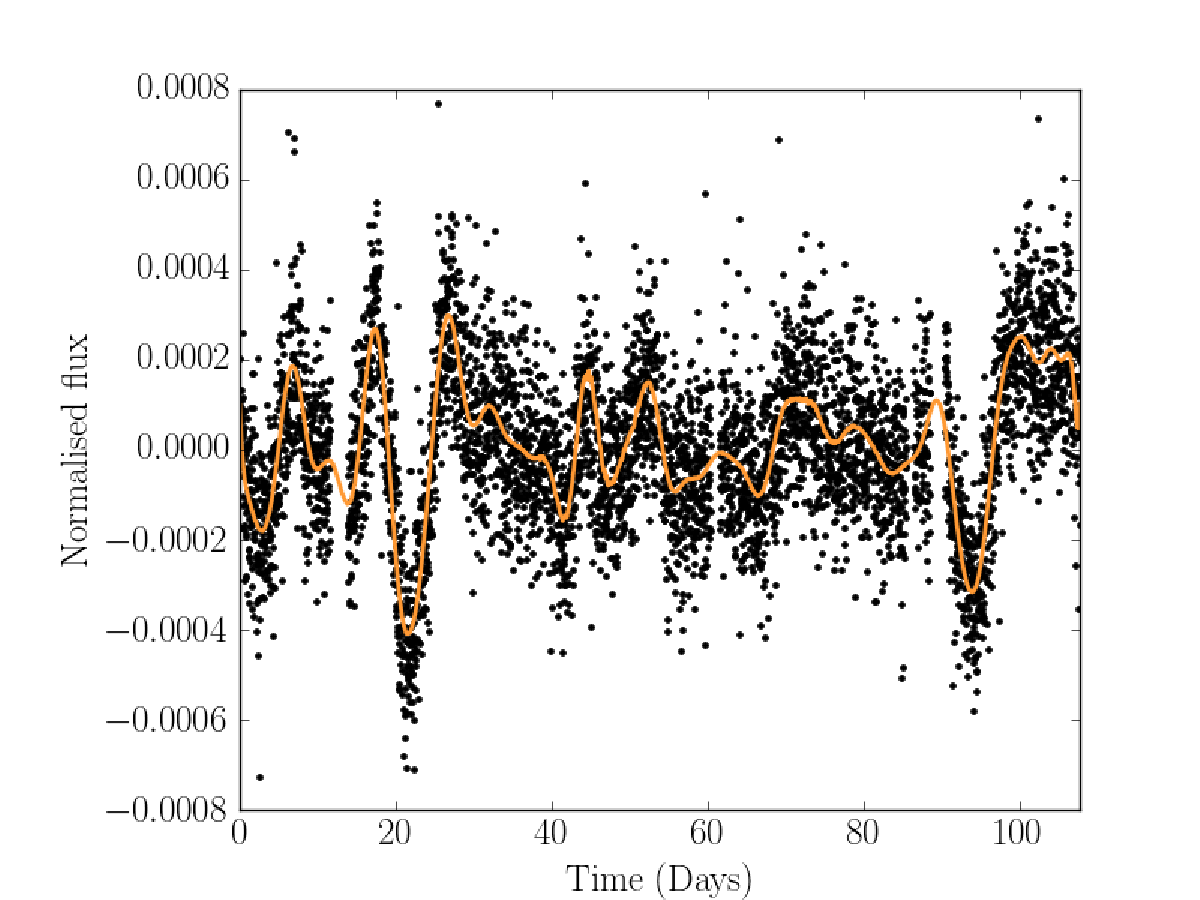
\includegraphics[width=6in, clip=true]{figures/Kepler452b.pdf}
% \caption[A light curve with a GP model.]
% {Light curve of Kepler-452 b, a habitable-zone, Earth-sized planet
% hosting G star \citep{Jenkins2015}. The orange line shows a fit to the data using
% a Gaussian process model with a QP covariance kernel function.}
% \label{fig:GP_example}
% \end{center}
% \end{figure}

\begin{figure}
\begin{center}
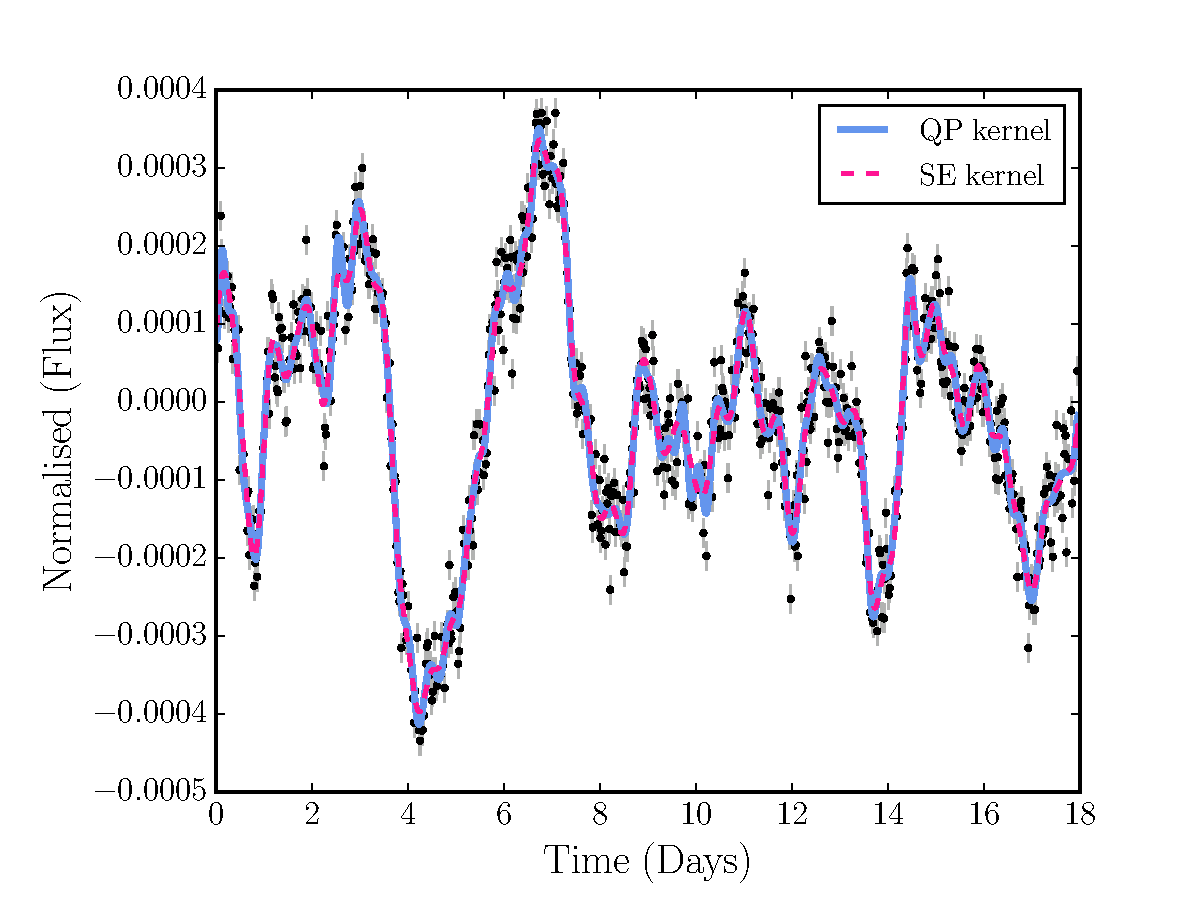
\includegraphics[width=6in, clip=true]{figures/001430163.pdf}
\caption[A light curve with a GP model.]
{Light curve of KID 1430163, an active star with a rotation period of $\sim$ 4
days.
The blue solid line shows a fit to the data using
a Gaussian process model with a QP covariance kernel function and the pink
broken line shows a fit with a SE kernel function.
Both kernel functions provide an adequate fit to the data, however we use the
QP function because it has a useful parameter that corresponds to the star's
rotation period.}
\label{fig:GP_example}
\end{center}
\end{figure}

\section{Rotation period injection and recovery}

In order to test the GP method we attempted to the measure rotation periods of
a set of simulated light curves.
We simulated \nlightcurves\ light curves using a spot model similar to that
used
% We used light curves simulated
for the \citet{Aigrain2015} `hare and hounds' rotation period recovery
experiment.
These light curves were simulated by placing dark, circular spots with slowly
evolving size, on the surface of bright, rotating spheres, ignoring
limb-darkening effects.
\citet{Aigrain2015} simulated one thousand light curves in order to test the
ability of participating teams to recover both the stellar rotation periods
and the rotational shear: the amplitude of surface differential rotation.
% Since we are not interested in recovering differential rotation we only used
% those light curves simulated {\it without} differential rotation, of which
% there are \nlightcurves.
Unlike in their study we are not interested in recovering differential
rotation in this work, so did not include it in our simulations.
We opted to use only solid-body rotators because differential rotation may
produce some additional scatter in the rotation period measurements recovered.
This code can also be adjusted to produce more realistic light curves by
altering spot lifetimes.
Stars with spot lifetimes that are long relative to their rotation periods
will have highly periodic light curves.
Those with short spot lifetimes will be more quasi-periodic.
We fixed the mean spot lifetime at an arbitrary value of 30.5 days for all
light curves in these initial tests.
In future we plan to include both differential rotation and variable spot
lifetimes in our light curve model.
Light curves were simulated with a real \Kepler\ long-cadence time array, with
one data point every thirty minutes over a four year duration.
The rotation periods of the simulations were randomly drawn from a log-uniform
distribution between 0.5-60 days.
Figure \ref{fig:noise-free_lc} shows an example of a simulated, noise-free
light curve with a period of 17.4 days.

% The ranges and distributions of the physical stellar parameters used in the
% simulated light curves are tabulated below, in table
% \ref{tab:simulation_parameters}.

% \begin{table*}
% \begin{center}
% \caption{Ranges and distributions of parameters used to simulate light curves
% in \citet{aigrain2015}}
% \begin{tabular}{lcc}
% \hline\hline
%     Parameter & Range & Distribution \\
%     \hline
%     Rotation period, $P_{rot}$ & 10 - 50 days (90\%) & log uniform \\
%     & 1 - 10 days (10\%) & log uniform \\
%     Activity cycle length & 1 - 10 years & log uniform \\
%     Inclination & 0 - 90$^\circ$ & Uniform in $\sin^2i$ \\
%     Decay timescale & (1 - 10) $\times P_{rot}$ & log uniform \\
% \hline
% \end{tabular}
% \end{center}
% \end{table*}
% \label{tab:simulation_parameters}

% and figure \ref{fig:period_hist} shows the
% distribution of rotation periods in the \citet{aigrain15} sample.
% \begin{figure}
% \begin{center}
% 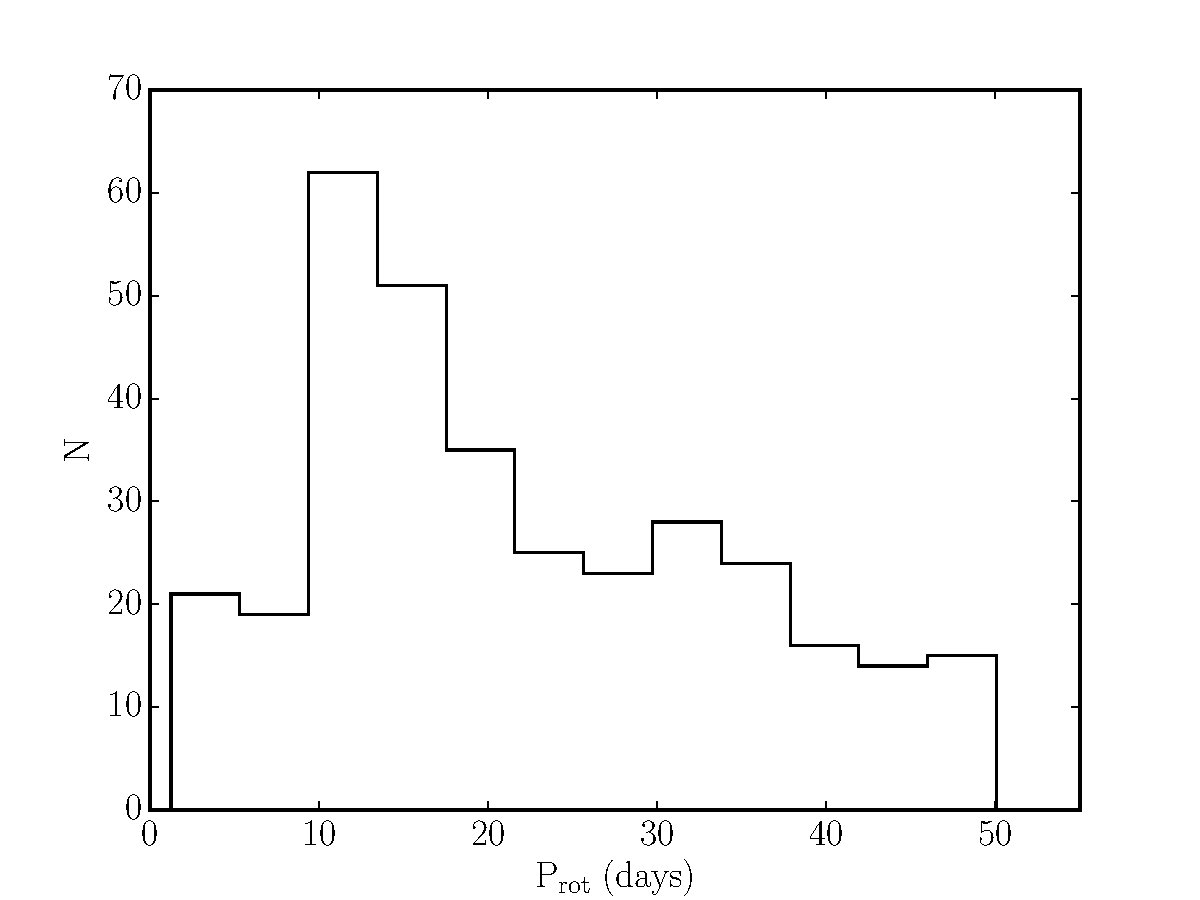
\includegraphics[width=6in, clip=true]{figures/acf_compare_noise-free_hist.pdf}
% \caption{A histogram of the rotation periods used to generate the simulated
% light curves in \citet{aigrain15}.}
% \label{fig:period_hist}
% \end{center}
% \end{figure}

\begin{figure}
\begin{center}
% 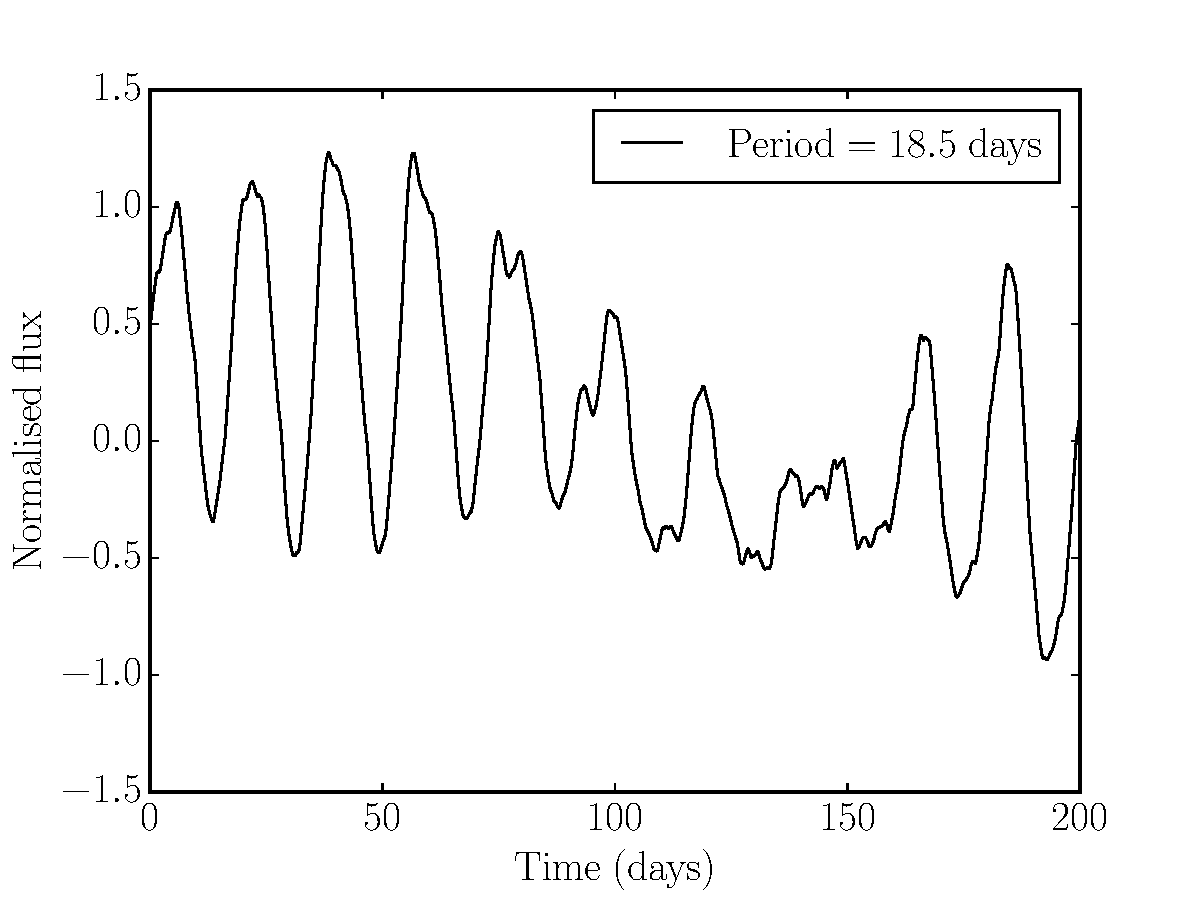
\includegraphics[width=6in, clip=true]{figures/noise-free_lc.pdf}
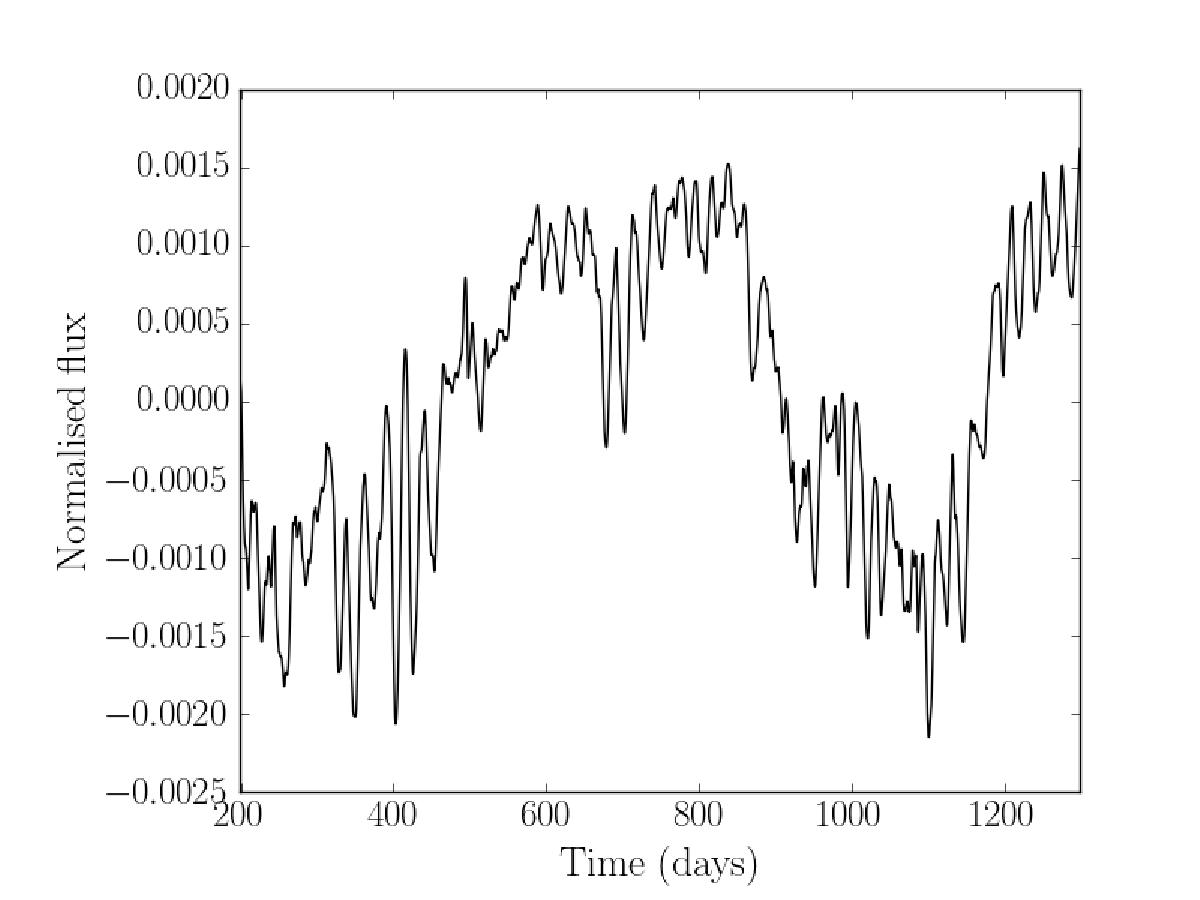
\includegraphics[width=6in, clip=true]{figures/thesis_plot.pdf}
\caption[A simulated light curve.]
{An example simulated, noise-free light curve. This `star' has a
rotation period of 17.4 days.}
\label{fig:noise-free_lc}
\end{center}
\end{figure}

Initial tests were conducted on noise-free light curves, in order to provide
proof-of-concept.
We attempted to recover the rotation periods of these \nlightcurves\ light
curves
% , both with and without noise, (\ie before {\it and} after being injected
% into \kepler light curves)
using three rotation period recovery methods: the ACF method, the LS
periodogram method and the GP method.

\subsection{ACF}

We calculated an ACF for each light curve using the method of
\citet{Mcquillan2013}.
In this method, an ACF is calculated for each light curve and smoothed by
convolving with a Gaussian with $\sigma=9$ days.
A rotation period is estimated as the lag-time of the first peak in the ACF,
unless the second peak is larger in which case {\it that} lag-time is
interpreted as the true period.
The second peak in an ACF can be larger than the first if there are two active
regions at or near opposite longitudes on the surface of the star---this would
produce a light curve with two dips per rotation period.
% By extension, if three active longitudes existed at 60$^\circ$ separations on
% the stellar surface, the first peak in the ACF may be at one third of the true
% rotation period and so on.
An example ACF of the light curve in figure~\ref{fig:noise-free_lc} is shown
in figure \ref{fig:ACF_example}.

\begin{figure*}
\begin{center}
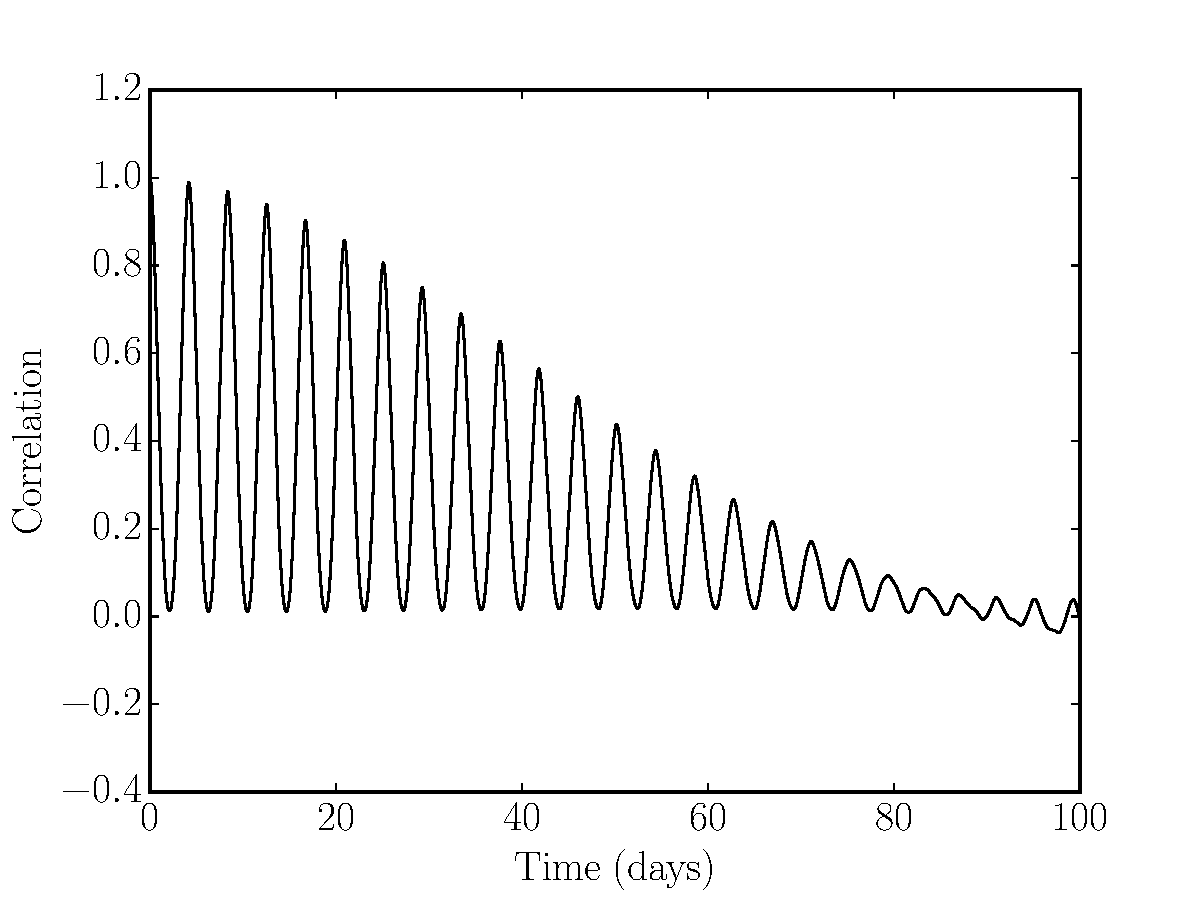
\includegraphics[width=6in, clip=true]{figures/noise-free_acf.pdf}
\caption[An ACF of a simulated light curve.]
{The autocorrelation function of the simulated, noise-free light
curve depicted in figure \ref{fig:noise-free_lc}.}
\label{fig:ACF_example}
\end{center}
\end{figure*}

The ACF method has proven to be extremely useful for measuring rotation
periods.
The catalogue of rotation periods of \Kepler\ stars provided in
\citet{Mcquillan2013} has been widely used by the community and has provided
ground-breaking results for stellar and exoplanetary science.
The results of the ACF method as tested in \citet{Aigrain2015} were positive
(see, for example their figure 8) as it produced a large number of accurate
rotation period measurements.
Another advantage of the ACF method is that it is conveniently fast to
implement.

We applied the ACF method to our sample of \nlightcurves\ noise-free,
simulated light curves.
Periods measured using the ACF method are plotted against the original
rotation period values used to generate the light curves in figure
\ref{fig:compare_noise_free}.
% 73\% of the injected rotation periods were recovered with a value lying
% within 10\% of the truth and 83\% within 20\%.
A noteworthy feature of this figure is that many of the points fall below the
$x=y$ line, \ie\ the recovered rotation periods are a little shorter than the
true periods.
We believe this is a feature of the peak position measurement method that is
performed on the ACF.
ACFs of stellar light curves can be roughly described as a cosine function
super-imposed on top of a decaying exponential.
In such a function the peak positions can be shifted towards the left--the
short period end--because the decaying exponential raises the left side of
each peak more than the right.
It is possible to model this effect of course, however the standard practice
is to simply measure the peak position without taking it into account.
We are still investigating the origin and implications of this effect.
% To demonstrate that this effect reproduces the underestimated periods seen in
% figure \ref{fig:compare_noise_free}, we simulated 1000 ACFs by generating
% cosine plus exponential functions with a range of periods, decay timescales
% and relative amplitudes.
% The measured position of the first peak in each simulated ACF is compared to
% the true position in figure \ref{fig:exp_sine_test}.
% The same underestimation of the peak position is apparent in this figure.
% Dashed lines show harmonics of $2P_{\mathrm{rot}}$ and $1/2P_{\mathrm{rot}}$.
% In several cases, twice the true rotation period is measured.
% The RMS of residuals is 1.59 days.

% \begin{figure*}
% \begin{center}
% 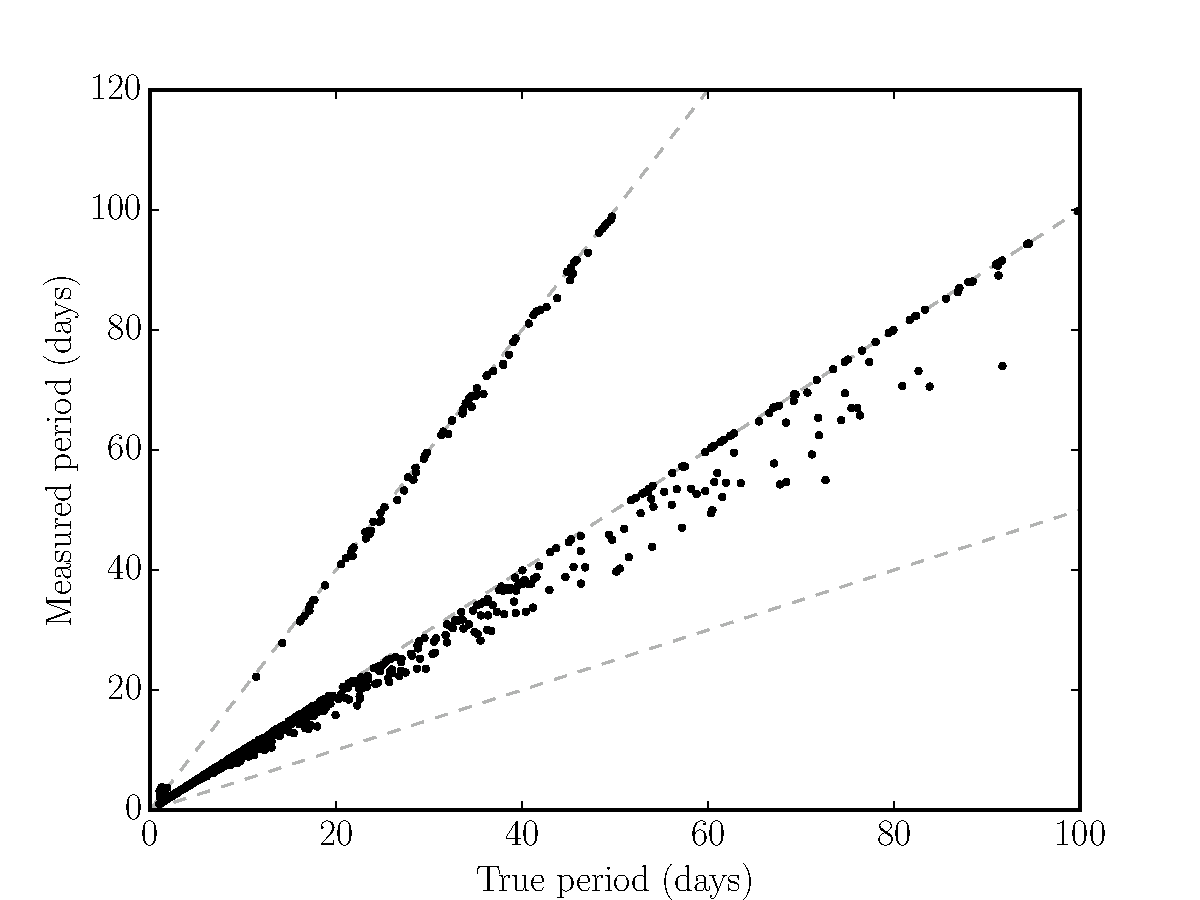
\includegraphics[width=6in, clip=true]{figures/exp_sine_test.pdf}
% \caption[A flaw in the ACF method.]
% {Recovered peak position as a function of the `true' period used to
% generate simulated ACFs. In many cases the position is measured short-wards of
% the truth, as also seen in figure \ref{fig:compare_noise_free}. The dashed
% lines are at $x=2x$, $x=x$ and $x=\frac{1}{2}x$.}
% \end{center}
% \end{figure*}
% \label{fig:exp_sine_test}

\begin{figure*}
\begin{center}
% 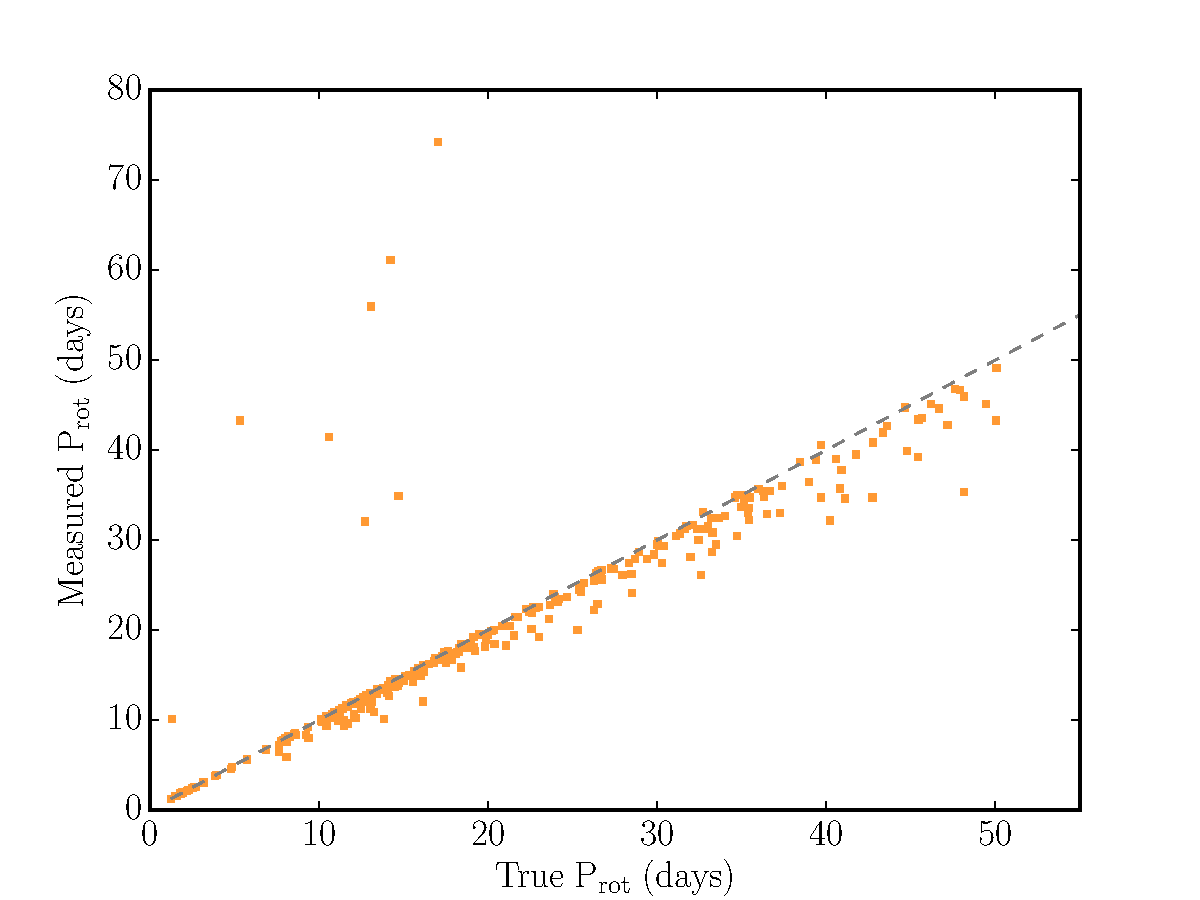
\includegraphics[width=6in, clip=true]{figures/acf_compare_noise-free.pdf}
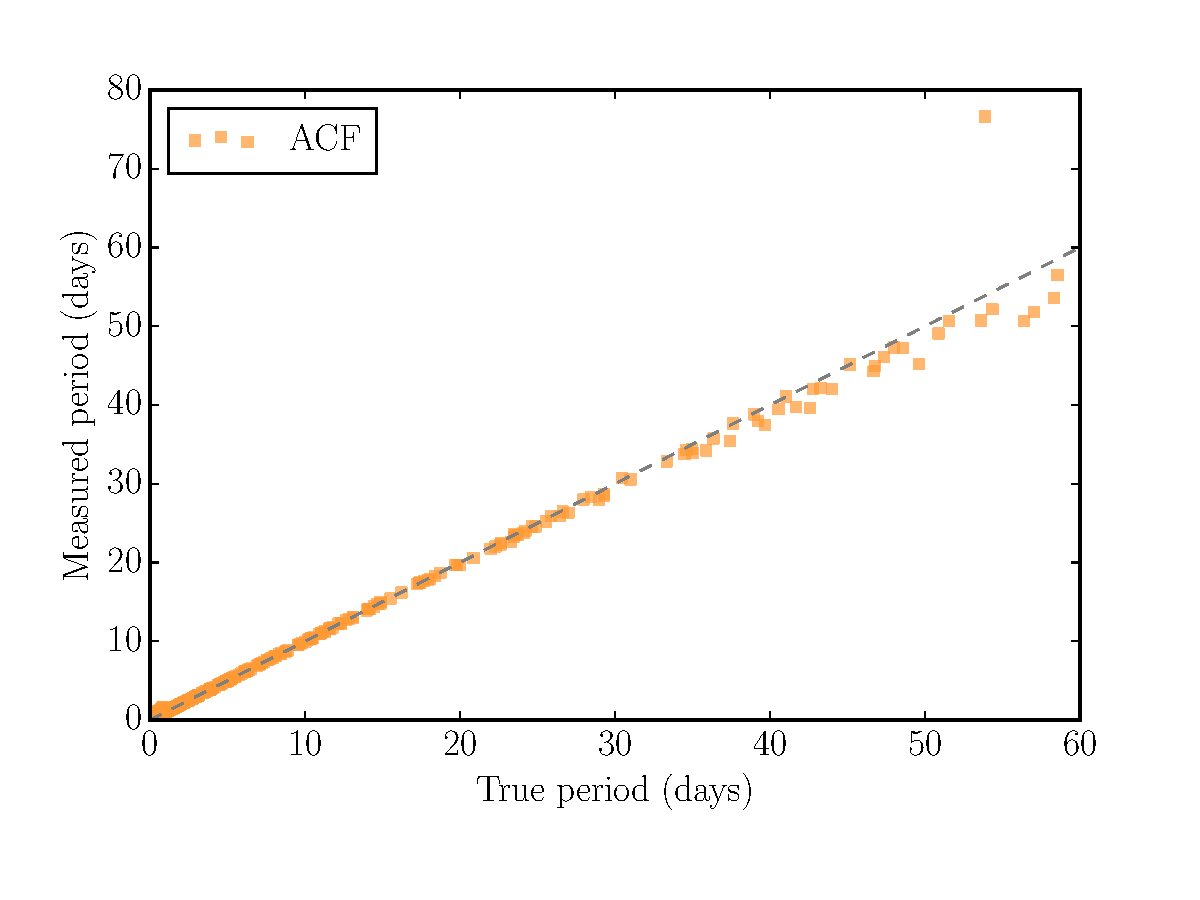
\includegraphics[width=6in, clip=true]{figures/compare_acf.pdf}
\caption[ACF results.]
{Rotation periods measured using the ACF method as a function of the
`true' period used to generate \nlightcurves\ simulated, noise-free light
curves.}
\label{fig:compare_noise_free}
\end{center}
\end{figure*}

\subsection{The sine-fitting periodogram method}

For each simulated light curve, a Lomb-Scargle (LS) periodogram
\citep{Lomb1976, Scargle1982} was computed over a grid of 10,000 periods,
evenly spaced in frequency, between 1 and 100 days.
The period of the highest peak in the periodogram was adopted as the rotation
period.
The resulting recovered rotation periods are plotted as a function of the true
periods in figure \ref{fig:pgram_compare_noise_free}.
These recovered rotation periods are in general more accurate than the ACF
results: they do not systematically over or under predict rotation period.
They are however less precise than the ACF results---the 8.03 day RMS of
residuals is five times larger.
% We believe that the unsuccessful recoveries occurring preferentially for
% shorter rotation periods are produced by additional, longer timescale
% variations in some of the light curves.
% Specifically, by fluctuations produced by changes in the total spot coverage
% on the stellar surface.
% These fluctuations can occasionally be larger in magnitude than those produced
% by the rotational signal itself and are present in the majority of outlying
% light curves that occupy the top left of figure
% \ref{fig:pgram_compare_noise-free}.

\begin{figure*}
\begin{center}
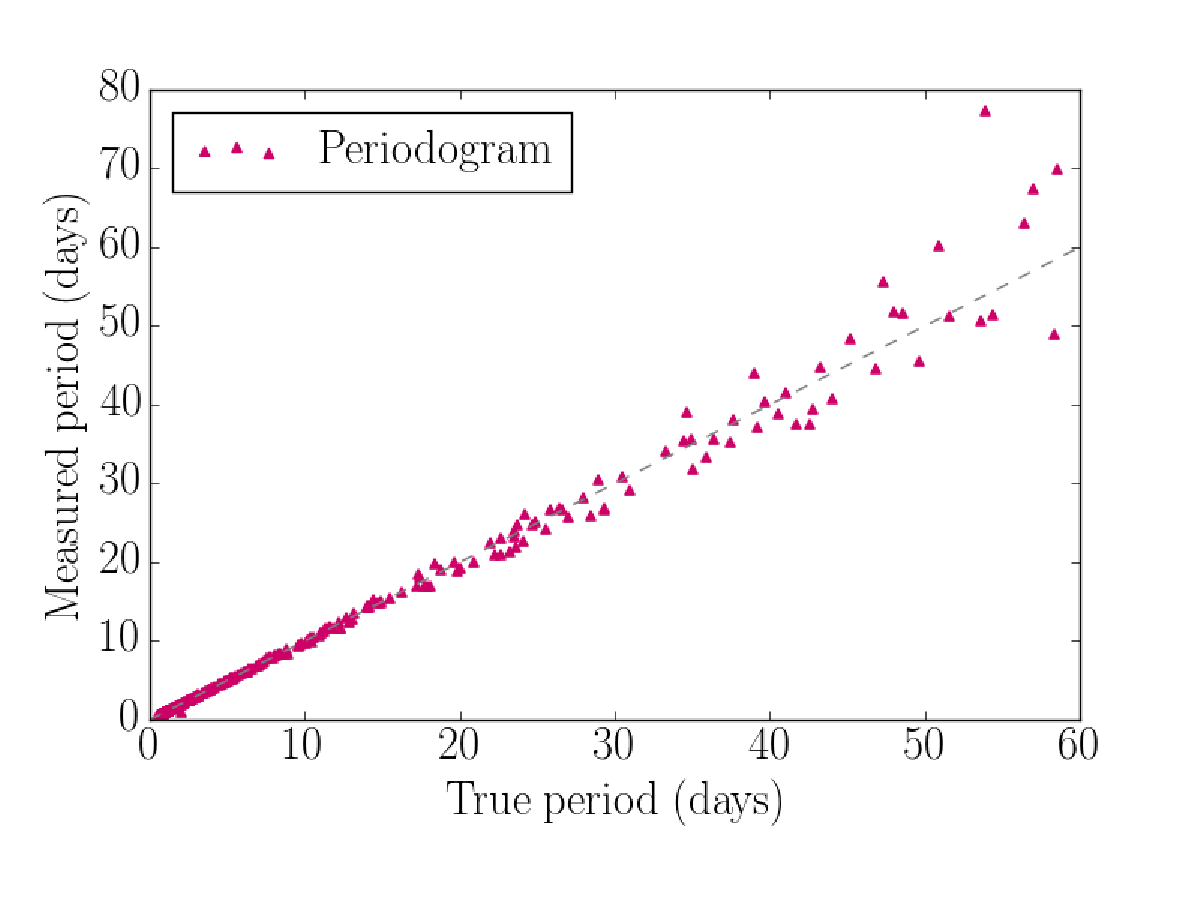
\includegraphics[width=6in, clip=true]{figures/compare_pgram.pdf}
\caption[LS periodogram results.]
{Rotation periods measured using the LS periodogram method as a
function of the `true' rotation period used to generate \nlightcurves\
simulated light curves.}
\label{fig:pgram_compare_noise_free}
\end{center}
\end{figure*}

\subsection{The GP method}

In order to recover the rotation periods of the simulated light curves using
Gaussian processes, we sampled the posterior PDFs of the kernel
hyperparameters described in equation \ref{eq:QP}.
The likelihood function for a GP is similar to the simple Gaussian likelihood
function that is used for optimisation problems where the uncertainties are
Gaussian and uncorrelated.
The latter can be written
\begin{equation}
\ln \mathcal{L} = -\frac{1}{2}\sum_{n=1}^N\frac{(y_n-\mu)^2}{\sigma_n^2}
    - \frac{N}{2}\ln(2\pi\sigma_n^2),
\end{equation}
\label{eq:chi2}
where $y_n$ are the data, $\mu$ is the mean model and $\sigma_n$ are the
Gaussian uncertainites on the data.
The equivalent equation in matrix notation is
\begin{equation}
\ln \mathcal{L} = -\frac{1}{2}\bf{r}^T\bf{C}^{-1}\bf{r}-\ln|\bf{C}|
    + \mathrm{constant},
\end{equation}
\label{eq:lhf1}
where $\bf{r}$ is the vector of residuals and $\bf{C}$ is the covariance
matrix,
\begin{eqnarray}
	\mathbf{C} &=& \left (\begin{array}{cccc}
	\sigma^2_1 & \sigma_{2, 1} & \cdots & \sigma_{N, 1} \\
	\sigma_{1, 2} & \sigma^2_2 & \cdots & \sigma_{N, 2} \\
    && \vdots & \\
	\sigma_{1, N} & \sigma_{2, N} & \cdots & \sigma^2_N
\end{array}\right )
\end{eqnarray}
In the case where the uncertainties are uncorrelated, the noise is `white',
(which is a frequent assumption made by astronomers and is sometimes
justified) and the off-diagonal elements of the covariance matrix are zero.
However, in the case where there is evidence for correlated
`noise'\footnote{In our case the `noise' is actually the model!}, as in the
case of \Kepler\ light curves, those off-diagonal elements are non-zero.
With GP regression, a covariance matrix generated by the kernel function,
${\bf K}$ replaces ${\bf C}$ in the above equation.
Incidentally, this approach is the reverse of the regression techniques
usually employed by astronomers.
In most problems in astronomy one tries to infer the parameters that describe
the mean model and, if correlated noise is present, to marginalise over that
noise.
Here, the parameters describing the correlated noise are what we are
interested in and our mean model is simply a straight line at $y=0$.

One could either maximise this likelihood function in order to find the
best-fit hyper-parameters of the covariance kernel function or, as in our
approach, sample from the posterior PDFs of the hyper-parameters.
The advantage of the maximum-likelihood method is that the best-fit parameters
will be found much faster, but the uncertainities on the rotation period
will not be constrained.
In order to measure accurate uncertainties, the posterior PDFs of the
parameters must be explored.
Since obtaining accurate uncertainties on rotation periods is one of our main
motivations for this method, we use MCMC despite the added computational
expense.

We use the ACF period as an initial guess for the rotation period (this
decision is discussed further in section \textsection \ref{sec:discussion}).
We use a uniform prior over rotation period with bounds described below and
assert that the covariance decay timescale parameter, $l$ must be greater than
the rotation period.
This represents our assumption that the evolution timescale of active regions
is greater than stellar rotation periods.
This assumption may be more valid for late spectral types---hot stars have
smaller active regions which are likely to be shorter-lived.
For the remaining hyperparameters we use the following initial values and
log-uniform prior distributions:
\begin{eqnarray}
 	&	A_{initial} = e^{-5}, \sim \exp(U[-20:20]) \\ \nonumber
 	&	l_{initial} = e^{7}, \sim \exp(U[-20:20]), l<P \\ \nonumber
 	&	\Gamma_{initial} = e^{0.6}, \sim \exp(U[-20:20]) \\ \nonumber
 	&	\sigma_{initial} = e^{-16}, \sim \exp(U[-20:20]) \\ \nonumber
 	&	P_{initial} = P_{ACF}, \sim U([1 - 0.4]P_{ACF}<P_{ACF}<[1 +
0.4]P_{ACF}).
 \end{eqnarray}
 \label{eq:initialisation}
$\sigma$ is an additional white noise term added to the diagonal elements of
the covariance matrix. It is the fraction by which the observational
uncertainties have been underestimated.
If the errorbars reported on the data are too small, this parameter will be
non-zero.
In practice this parameter should always be non-zero when performing GP
regression.
This is because the covariance matrix must be positive definite, however
matrix inversion performed using most solvers is approximate, not exact,
therefore slight deviations from positive definitism can arise.
Including a small amount of extra variance in the model allows enough
flexibility that the matrix inversion algorithms do not run into numerical
issues.

We subsampled the light curves in order to reduce computation time.
The subsampling is altered for each light curve and depends, again, on the ACF
period estimate.
We found that retaining only 20 data points per rotation period, based on the
ACF period estimate, significantly reduced computation time whilst maintaining
performance.
The {\tt george} \citep{George} python package was used to implement the GP
model which uses the fast matrix solver, HODLR \citep{Ambikasaran2014}.
Matrix operations performed with HODLR scale as $N \log ^2 (N)$, where $N$ is
the number of data points.
We used {\tt emcee} \citep{Foreman-Mackey2013}, an affine invariant ensemble
sampler to explore the posterior PDFs of the model parameters.
The rotation period was taken as the median value of the posterior PDF.
The resulting measured rotation periods are compared to the true rotation
periods in figure \ref{fig:GP_compare_noise_free}.
The root-mean-square (RMS) of residuals for the GP results is 0.26 days.
The results of all three methods are plotted on the same axes in figure
\ref{fig:compare_noise_free}.

% The subsampling reduces computation time simply by contracting the data

\begin{figure*}
\begin{center}
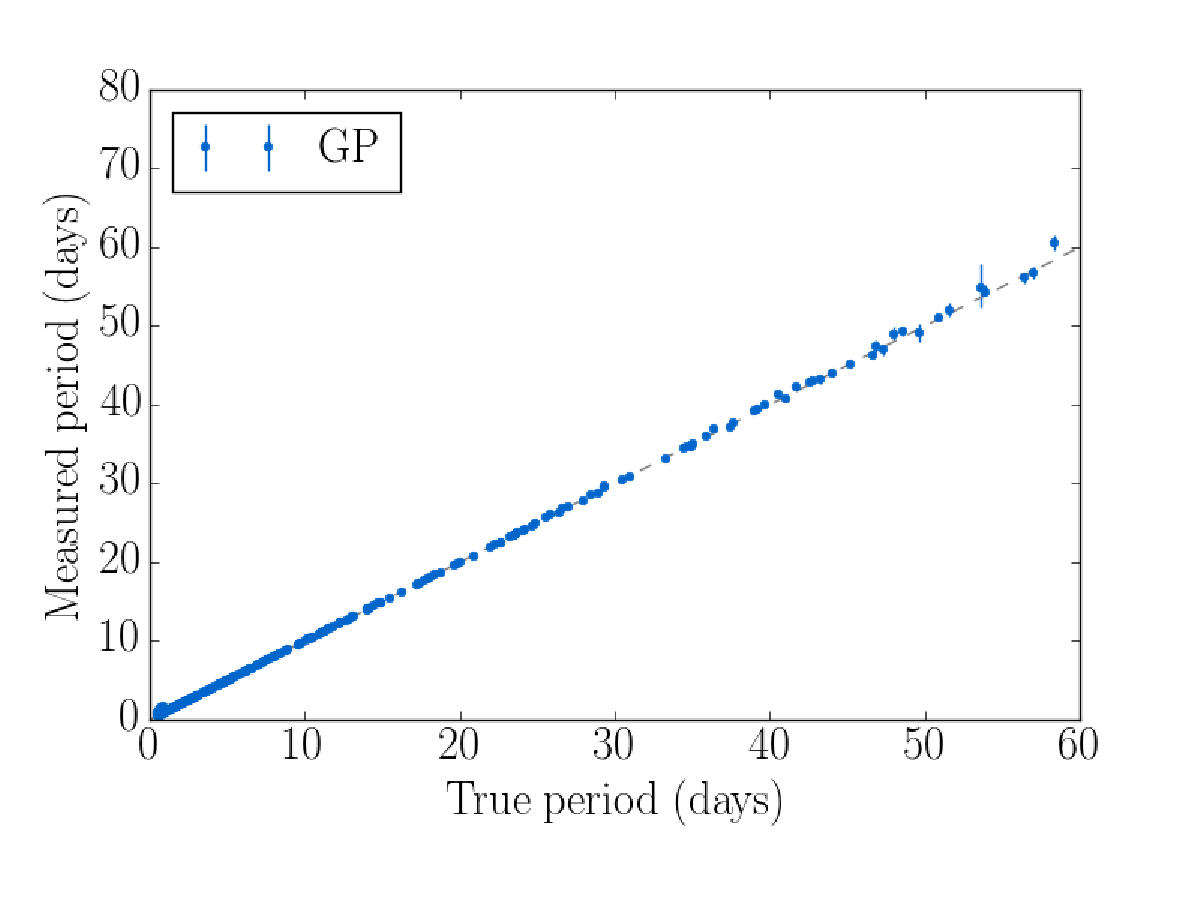
\includegraphics[width=6in, clip=true]{figures/compare_gp.pdf}
\caption[GP results.]
{Measured vs true rotation period for \nlightcurves\ simulated light
curves using the GP method.}
\label{fig:GP_compare_noise_free}
\end{center}
\end{figure*}

\begin{figure*}
\begin{center}
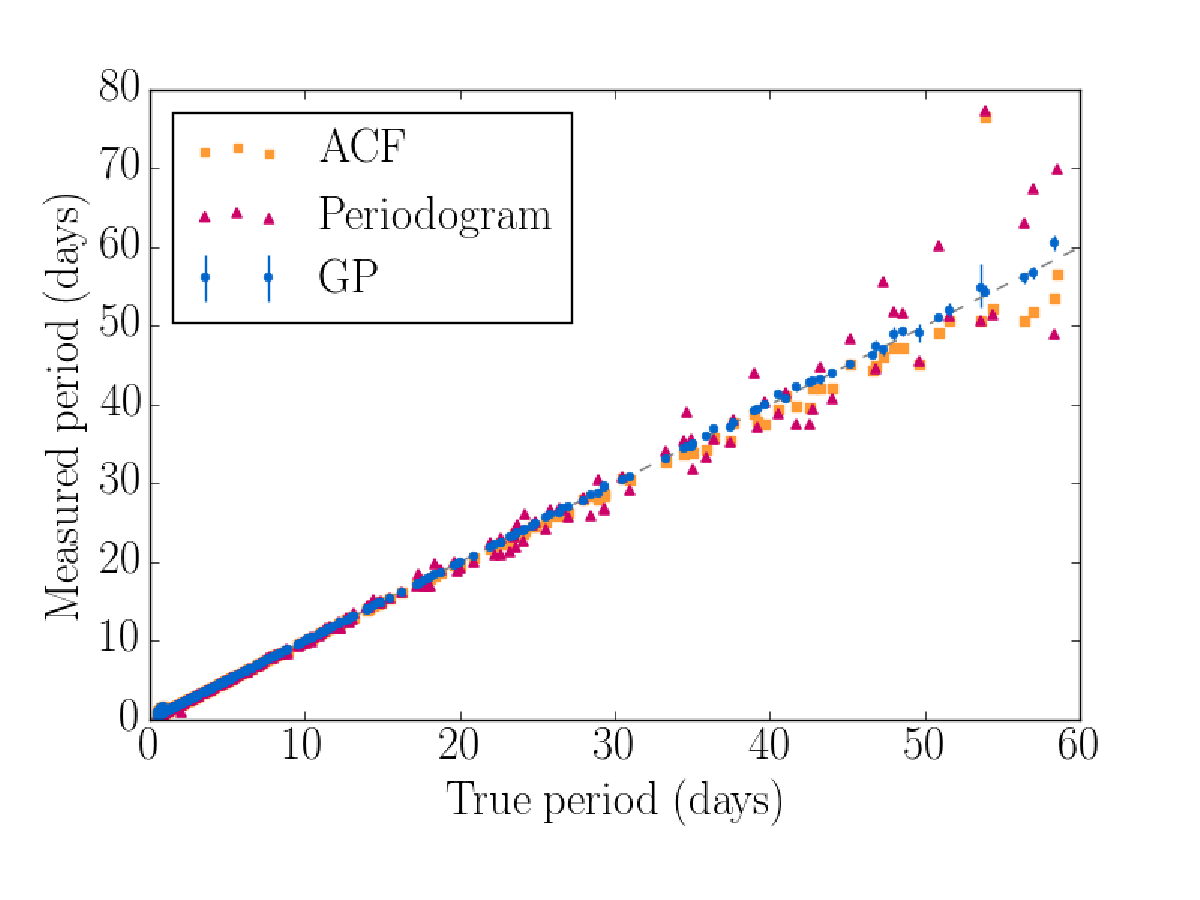
\includegraphics[width=6in, clip=true]{figures/compare2.pdf}
\caption[All results.]
{Measured vs true rotation period for \nlightcurves\ simulated light
curves from the three different methods described in the text.}
\label{fig:compare_noise_free}
\end{center}
\end{figure*}

The marginal posterior distributions of the QP kernel hyperparameters for an
example noise-free light curve  with a 14.4 day rotation period, are shown in
figure \ref{fig:gp_posteriors}.
The light curve itself with the best fit GP model is shown in figure
\ref{fig:demo_lc_GP}.

\begin{figure*}
\begin{center}
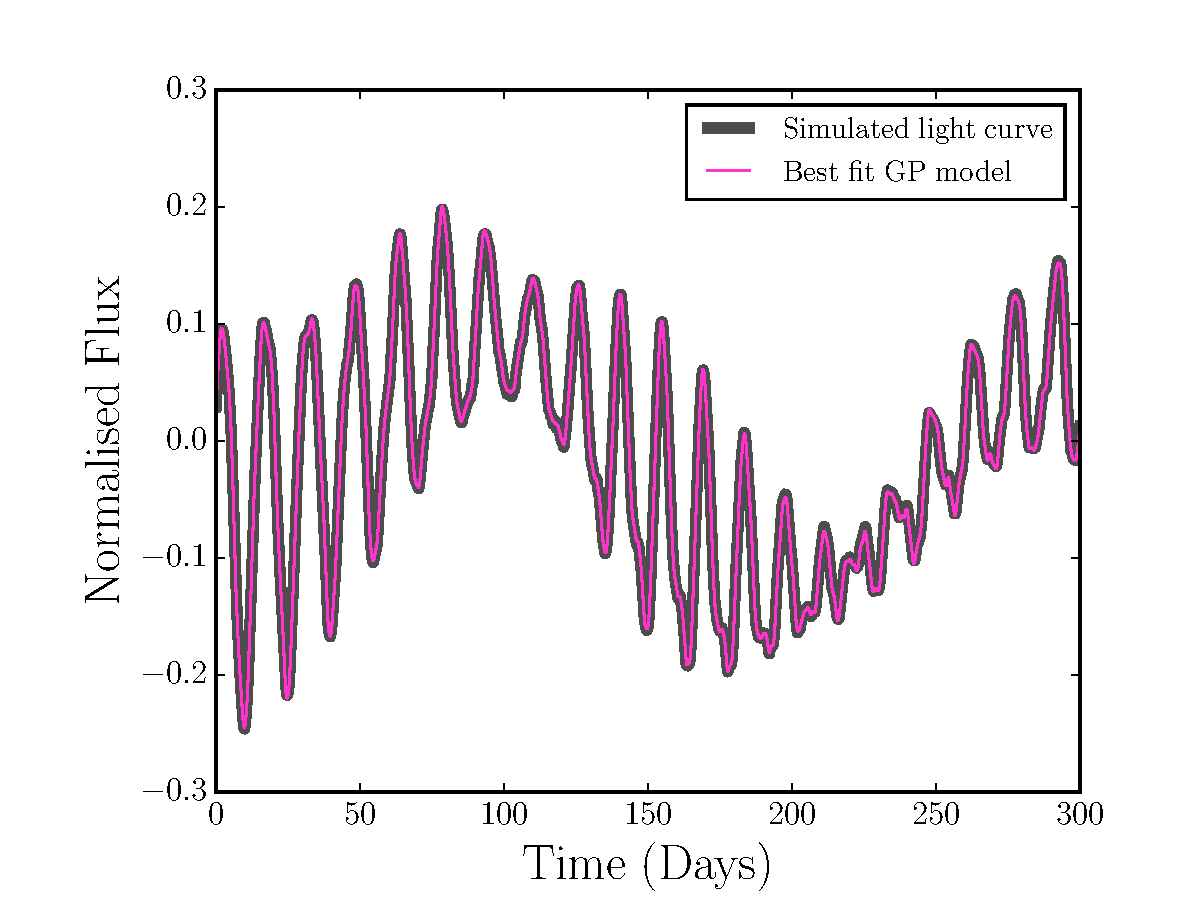
\includegraphics[width=6in, clip=true]{figures/demo_lc_GP.pdf}
\caption{A simulated light curve with a rotation period of 14.4 days.
The pink curve shows the GP model with the best-fit parameters.
The marginal posteriors of the GP hyper-parameters used to produce this fit
are shown in figure \ref{fig:gp_posteriors}.}
\label{fig:demo_lc_GP}
\end{center}
\end{figure*}

\begin{figure*}
\begin{center}
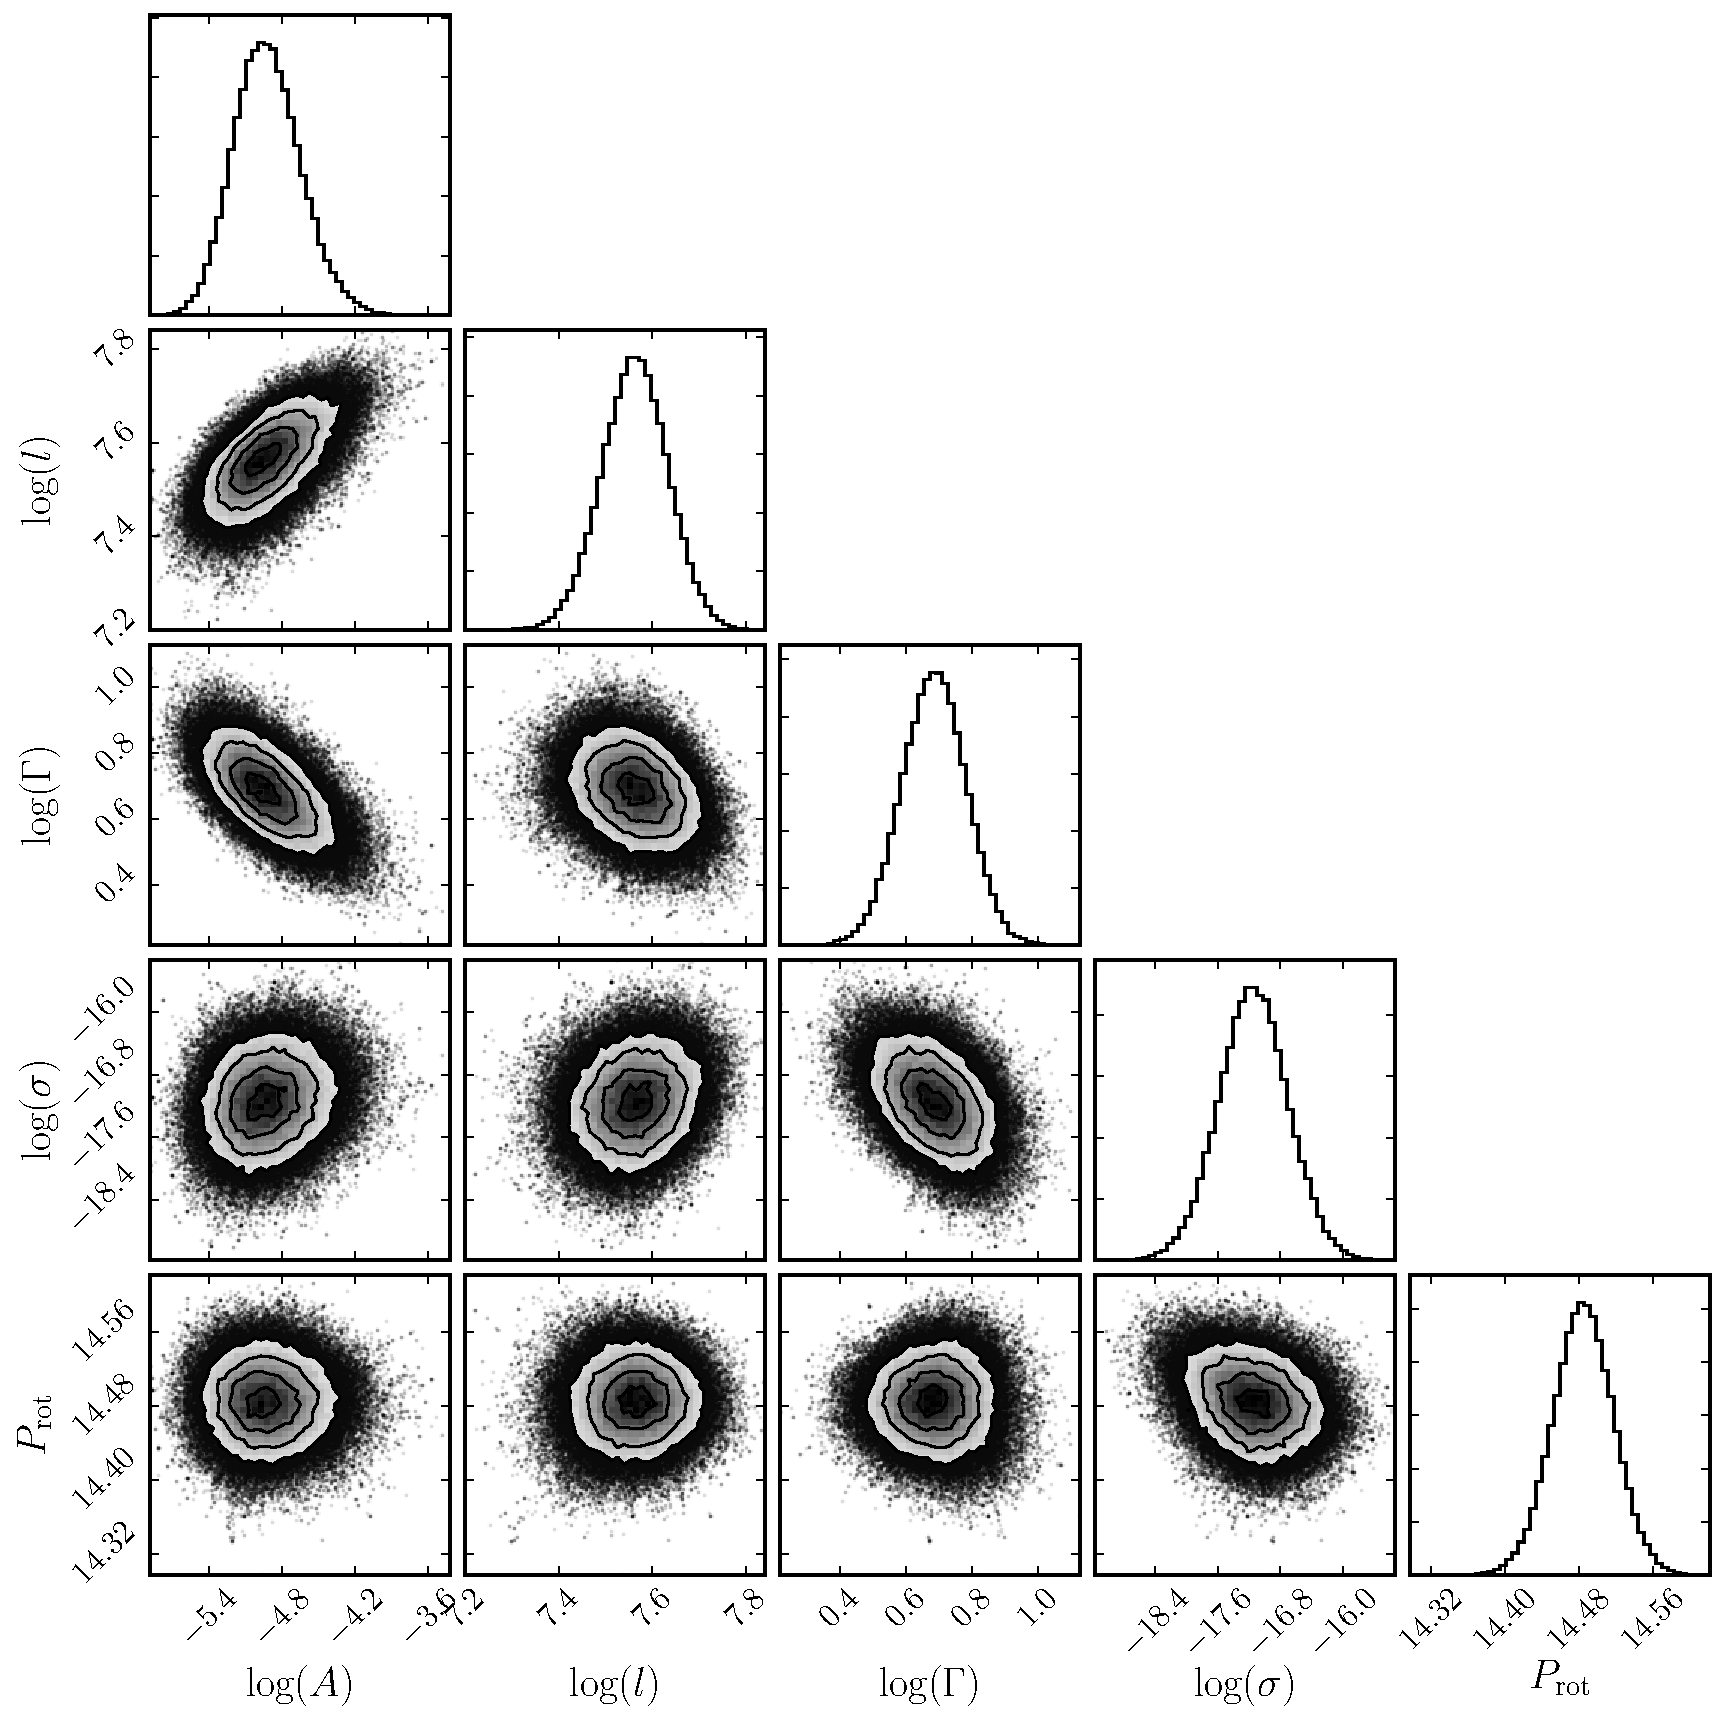
\includegraphics[width=6in, clip=true]{figures/demo_triangle.pdf}
\caption{Marginal posterior PDFs of the QP GP model parameters. $\sigma$ is an
additional white noise term added to the diagonal elements of the covariance
matrix. It is the fraction by which the observational uncertainties have been
underestimated. If the errorbars reported on the data are too small, this
parameter will be non-zero. Since this light curve was simulated without
noise, this parameter is very close to zero.
The true rotation period of this star is 14.4 days.}
\label{fig:gp_posteriors}
\end{center}
\end{figure*}

\subsection{Real \kepler\ data}

The noise-free light curves were injected into real \kepler\ light curves in
order to test the performance of the GP method in a realistic case.
Ideally, simulated light curves would have been injected into the \kepler\
pixel-level data, then the same detrending method that is applied to the
\kepler\ light curves would be applied to these light curves before attempting
to measure rotation periods for these stars.
However, since this work is designed to be more of a demonstration of the
overall efficacy of the GP periodogram, rather than the development of a
\Kepler\ specific method, this is beyond the scope of our demonstrations.

Unfortunately, automating the GP method so that it can run on large numbers of
real \kepler\ light curves is difficult.
The added noise reduces the acceptance fraction within the MCMC chains,
significantly increasing the required time for convergence.
Despite this, the method works well on individual targets where chains can be
run for a long time and subsampling can be reduced.
We used a simulated, noisy light curve from \citet{Aigrain2015} that was
generated by injecting a noise-free simulation into a real \kepler\ light
curve in order to preserve realistic \kepler\ noise properties.

\kepler\ light curves are big data and extracting the maximum amount of
information from them requires either large numbers of CPU hours, or using
work-arounds.
One feature of \kepler\ light curves that works to our advantage is that they
are naturally broken up into smaller time units by quarterly (three month)
breaks.
Splitting the data set into quarters, rather than modelling the entire time
series contiguously speeds up the computation time as inverting several
small matrices is faster than inverting one large one.
The \kepler\ quarter divisions are natural places to split the time series
because the spacecraft rotates by ninety degrees every quarter (three months),
placing each star on a new CCD module.
Pixel response functions and background flux differs from pixel-to-pixel and
module-to-module, so noise properties of \kepler\ light curves change every
quarter.
Additionally, changes in the spacecraft's orientation and position during
quarterly re-pointings temporarily affect the temperature of the CCD,
producing systematic features in the light curves at the start of some
quarters.
We model each quarter separately but the parameters of the GP kernel function
are global, {\it i.e.} we do not use a separate period parameter for each
quarter---there is just one period parameter for an entire light curve.
It would be possible to model the time series with a mixture of some global
parameters and some quarter-specific parameters, for example one might expect
that the amplitude of covariance, $A$ or white noise level, $\sigma$ to vary
on a quarterly basis.
However, since there are seventeen quarters this would lead to thirty-seven
parameters, and in the interest of minimising computation time (adding
parameters leads to longer MCMC burn in and convergence time), we choose to
use global parameters only.
Unfortunately, the application of this method to noisy test cases is still
under development and cannot provide results here.
We hope to develop this method further and apply it to real light curves in
the near future.

% The marginal posterior distributions of the QP kernel hyperparameters for an
% example noisy light curve  with a ... day rotation period, are shown in
% figure \ref{fig:gp_posteriors}.
% The light curve itself with the best fit GP model is shown in figure
% \ref{fig:demo_lc_GP}.

% \begin{figure*}
% \begin{center}
% 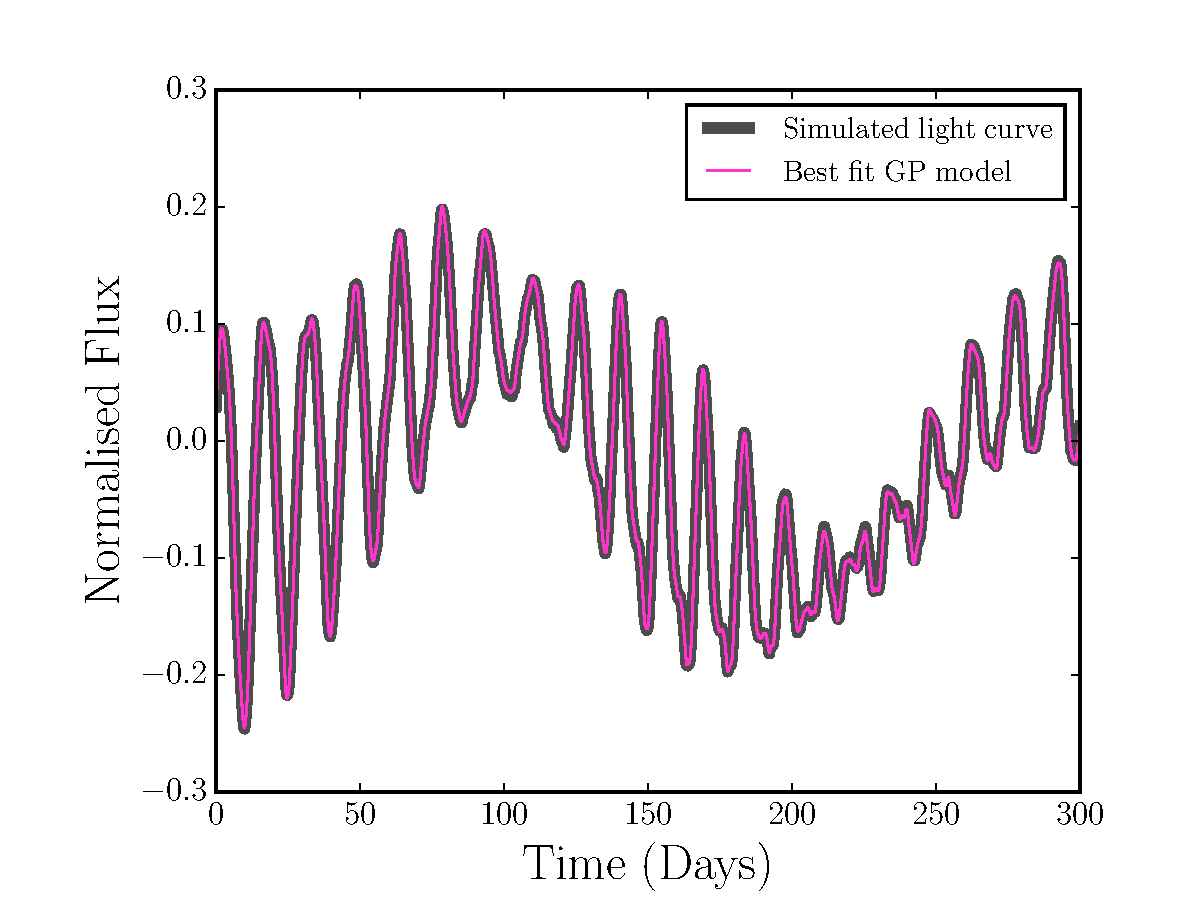
\includegraphics[width=6in, clip=true]{figures/demo_lc_GP.pdf}
% \caption{A simulated light curve with a rotation period of 14.4 days.
% The pink curve shows the GP model with the best-fit parameters.
% The marginal posteriors of the GP hyper-parameters used to produce this fit
% are shown in figure \ref{fig:gp_posteriors}.}
% \label{fig:demo_lc_GP}
% \end{center}
% \end{figure*}

% \begin{figure*}
% \begin{center}
% 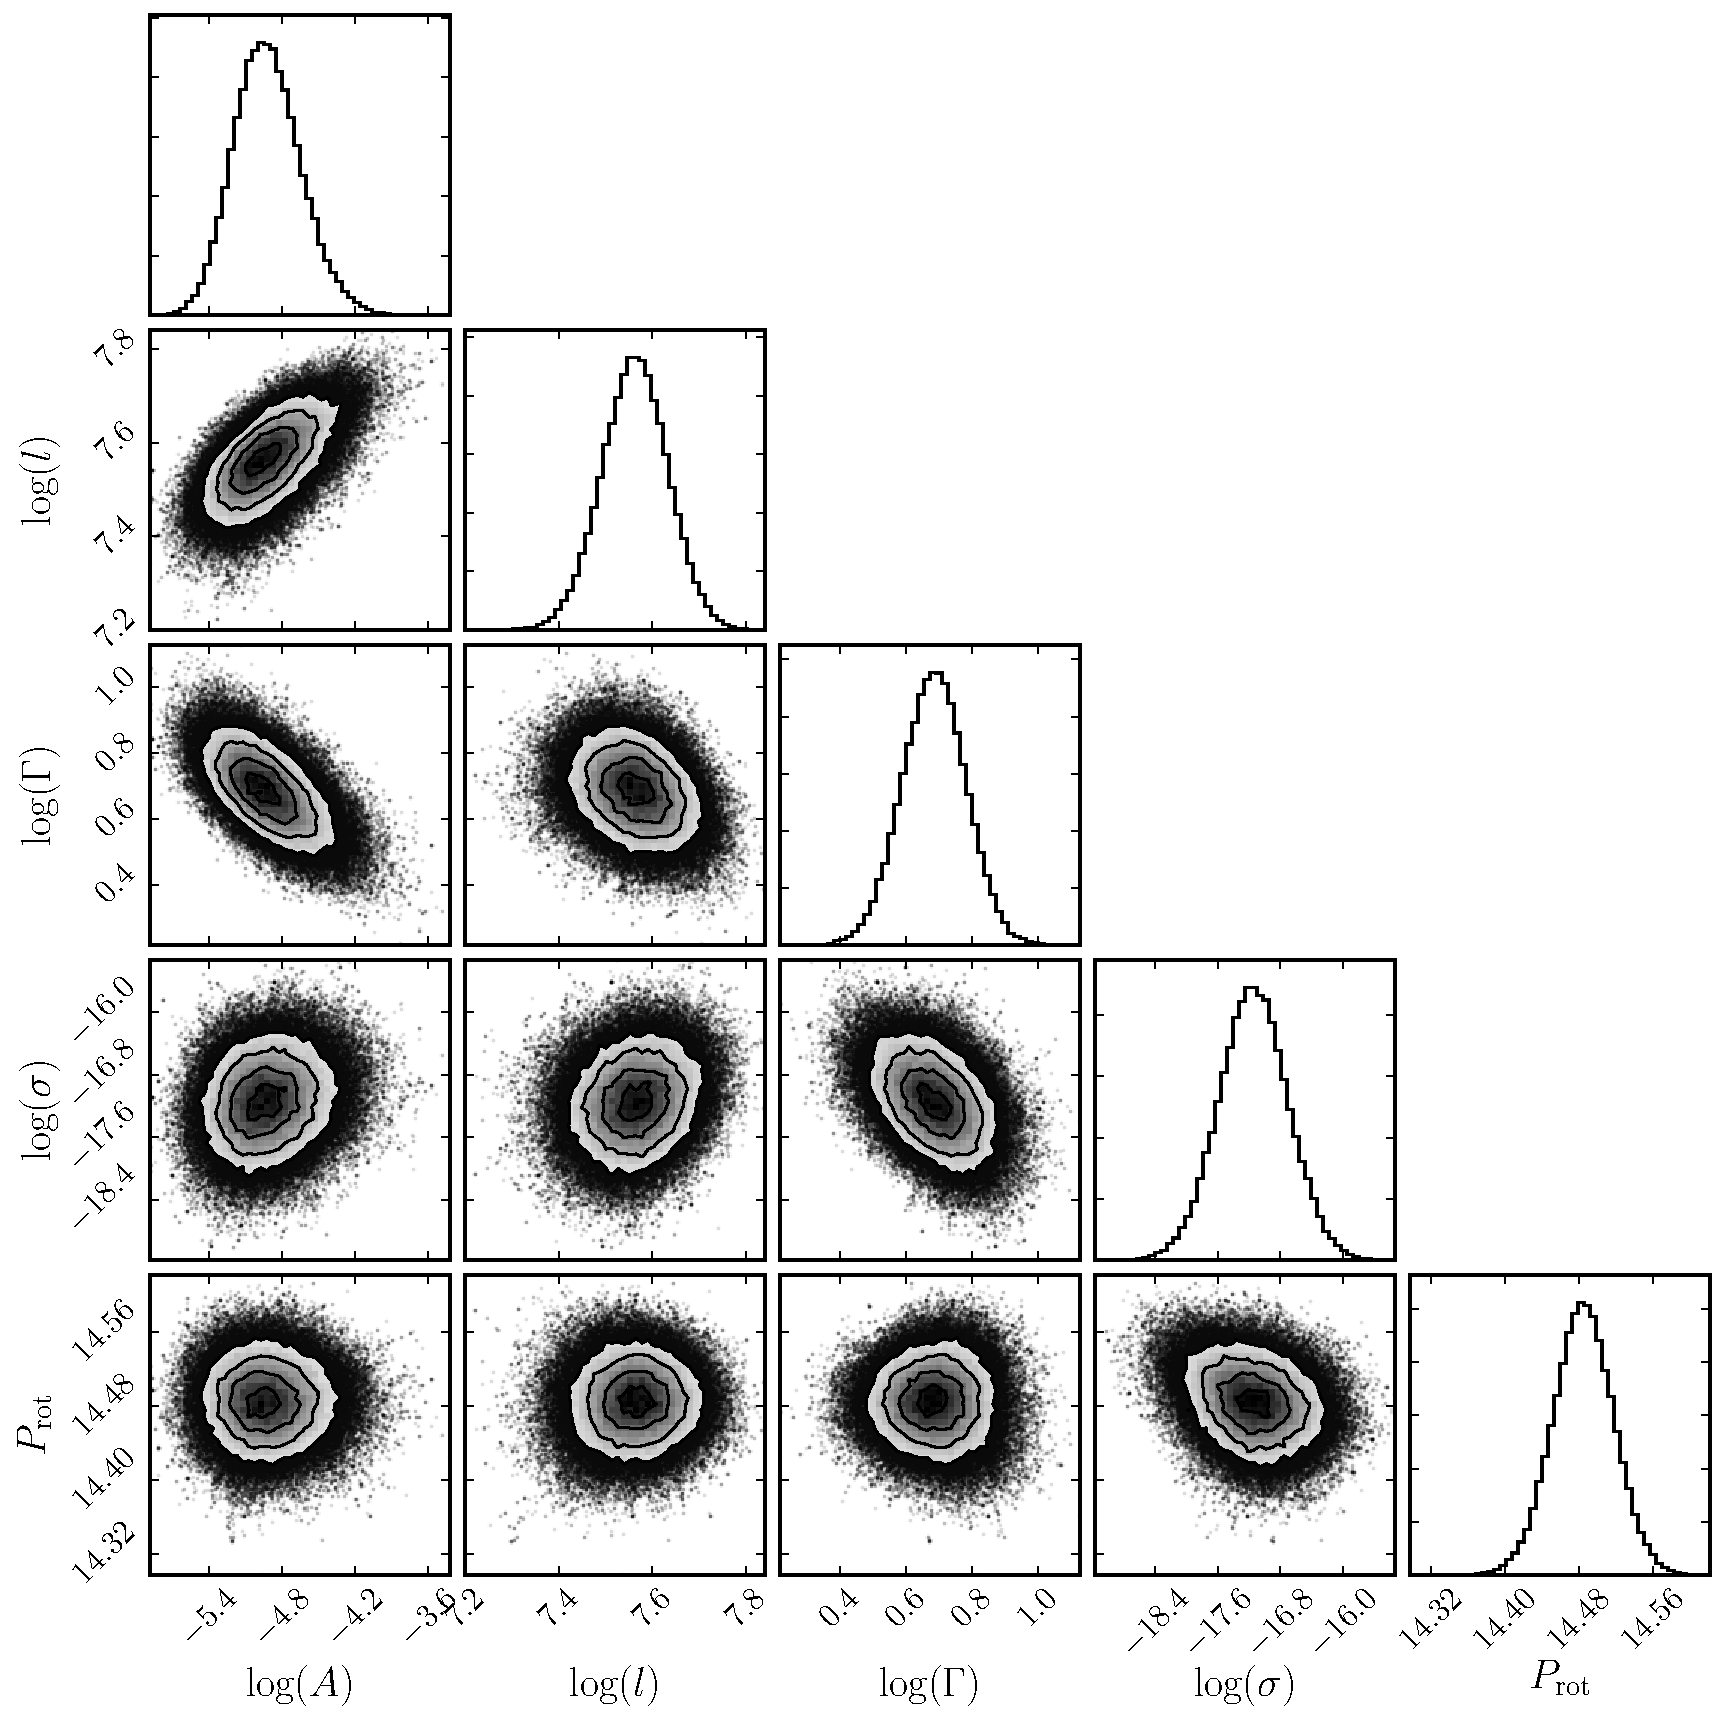
\includegraphics[width=6in, clip=true]{figures/demo_triangle.pdf}
% \caption{Marginal posterior PDFs of the QP GP model parameters. $\sigma$ is an
% additional white noise term added to the diagonal elements of the covariance
% matrix. It is the fraction by which the observational uncertainties have been
% underestimated. If the errorbars reported on the data are too small, this
% parameter will be non-zero. Since this light curve was simulated without
% noise, this parameter is very close to zero.
% The true rotation period of this star is 14.4 days.}
% \label{fig:gp_posteriors}
% \end{center}
% \end{figure*}

% \begin{figure*}
% \begin{center}
% \includegraphics[width=6in, clip=true]{figures/prediction.pdf}
% \caption{A noisy simulated light curve with a rotation period of 17.04 days.
% The blue curve shows the GP model with the best-fit parameters.}
% \end{center}
% \end{figure*}
% \label{fig:compare_noise_free}

\section{Discussion}
\label{sec:discussion}

The main drawback of the GP method is computation time.
Because GPs are so expensive to compute, it is necessary to come up with
shortcuts in order to perform inference on \kepler\ light curves, each of
which compromises accuracy.
The shortcuts that we employ here include:
\begin{itemize}
\item{Initialisation.
The choice of initial parameter values makes a difference to computation time:
the closer they are to the maximum likelihood parameters the shorter the MCMC
burn-in time.
Using the ACF period to initialise is not ideal as results will not be fully
independent of the ACF period unless MCMC chains are run for an infinitely
long time.} \item{Subsampling.
Not only is some information always lost by subsampling, but the choice of
subsampling frequency will also effect the results.
We chose to retain only 20 data points per period --- based on the ACF
period --- which, again means that our results are not independent of the ACF
results.}
\item{Priors.
We chose to use uniform, bounded priors to reduce parameter space and
therefore convergence time.
Unfortunately, if the true period lies outside the bounded region, it will
never be found.}
\end{itemize}

These shortcuts are only necessary when working with a large number of stars
(of order hundreds or thousands).
If only interested in single or small numbers of targets it may be possible to
reduce the extremity of these shortcuts or to avoid them altogether.

\subsection{The ACF method}
The main advantage of the ACF method over the GP method is speed: it is
extremely fast and therefore useful to get a quick estimate of a period.
We have demonstrated that the ACF method may produce rotation periods that are
slightly systematically biased towards lower rotation periods.
This effect comes from the process of extracting the period from the ACF
itself: typically superimposed onto a decaying exponential, that first peak in
the ACF gets shifted towards faster periods.
One may be able to get around this by modelling the ACF as a sum of a cosine
and exponential function (a similar function to GP kernel function) but
in practice ACFs tend to have a more complicated structure and it is not
possible to model them with a simple function.
This observation leads to the idea of modelling the ACF with a Gaussian
processes, which then logically progresses to a using a Gaussian process with
a Gaussian process kernel function.
Although this may be an attractive idea, in practice a GP would not
necessarily produce a positive semi-definite covariance kernel\footnote{One
that can be inverted; a necessary regression operation.}.
An alternative approach may be to correct for rotation period bias after the
peak position has been measured by inferring a correction factor.
Yet another approach could be to measure the mean separation between adjacent
peaks in the ACF: the first peak should be most strongly affected by the
exponential decay, the second peak less so, and so on.

\subsection{Initialisation}
Using the ACF to initialise the MCMC chains is not ideal because, of course,
one becomes reliant on the assumption that the ACF period is close to the true
period.
Of course, if you had infinite CPU time, this would not be a problem as you
would eventually sample the entire posterior PDF of the period parameter,
however in practice this is likely to be an issue.
The only way to get around this problem is to run the MCMC chains for as long
as possible, or, alternatively to use a sampler that is designed to move
around the parameter space much more quickly than {\tt emcee}; nested sampling
for example.
We chose to use the ACF periods rather than the periodogram periods to
initialise as, although there was some systematic bias present in these
results, that bias was small and there were fewer large outliers.

\subsection{Kernel function choice and interpretation of hyper-parameters}
The QP kernel function represents a simplistic effective model of a stellar
light curve.
It adequately describes the data, captures that all-important periodic quality
and is relatively simple, with only a few hyper-parameters.
It also satisfies the requirement to produce positive semi-definite covariance
matrices.
Whilst the QP kernel function evidently captures the periodic qualities of
light curves adequately, it is still a somewhat arbitrary choice.
Another valid choice would be a squared cosine function multiplied by a
squared exponential,
\begin{equation}
k_{i,j} = A \exp \left(-\frac{(x_i - x_j)^2}{2l^2}\right)
\cos^2\left(\frac{2\pi}{P}\right)
\end{equation}
\label{eq:cos_kernel}
This function produces a positive semi-definite matrix and has the $P$
parameter of interest.
It may in fact be even {\it more} suited to modelling stellar
light curves as it describes a Gaussian in frequency space.
It is easy to imagine a differentially rotating star with a period that is a
Gaussian in frequency space: the mean frequency would be the frequency at the
most active latitude, at or near which spots spend the majority of their time
and the tails would be occupied by spots that drift near the equator or poles.
The main difference between this cosine and the QP function is that the cosine
function allows negative covariances and the QP function does not.
Is is realistic to allow negative covariances?
In practice, the ACFs of \Kepler\ light curves often go negative.
However, many stars have two active regions on opposite hemispheres that
produce two brightness dips per rotation.
If the covariance is forced to be negative for two data points that are
separated by half a rotation period, those light curves with two peaks per
rotation period may not be well modelled.
It would be very worthwhile to test this assumption and this alternative
kernel function in future.
If CPU time were not limited there may be some benefit to performing formal
model comparison with different kernel functions.
However, the evidence integral is an ambitious calculation for models with
likelihood functions that take milliseconds to compute, let alone those
involving GPs with light curves containing thousands of data points which can
take minutes.

Clearly, stellar rotation periods are well represented by the $P$ parameter in
our QP kernel function, as evidenced by the its impressive ability to recover
the true rotation periods from the simulated light curves in this work.
However, it is not clear whether the QP kernel function is the {\it best}
function to use.
There may be an alternative function which is better suited to capturing
stellar variability and is able to recover periods even more precisely than
the QP kernel.
There may also be an alternative function which is more physically motivated,
that captures not just the rotation period but also (for example) the spot
lifetime or differential surface rotation.
This is beyond the scope of this work but we hope that these questions will be
answered in the near future.

\subsection{Future work}
The next stages of improving this method are listed as follows:
\begin{itemize}
\item{To optimise the tradeoff between computational efficiency and accuracy.
We have performed limited tests to explore the optimum subsampling strategy
and prior bounds.
These should be explored more thoroughly in future.
For example, it would be useful to know how the precision and accuracy of the
recovered rotation period varies as a function of subsampling frequency}
\item{To perform model selection with different kernel functions. Again, these
tests have not been performed due to the cost of calculating the fully
marginalised likelihood with GPs. This calculation may be prohibitively
expensive, however simpler model selection tests can be performed. For
example, the relative precision of rotation periods recovered using
alternative kernel functions could be tested.}
\item{To design and implement a physically motivated kernel function. We have
only explored the physical interpretation of one parameter in our kernel
function, $P$.
However, the other parameters may also be related to some physical processes.
For example, the overall timescale for covariance fall-off, $l$ may be
related to spot lifetimes.
A star with long spot lifetimes will show little variation in the overall
shape and amplitude of its light curve between rotations and $l$ will be
large.
In contrast, the light curve of a star with short spot lifetimes may display
non-repeating patterns and amplitudes that vary rapidly between rotations.
In this case $l$ will be small.
The $\Gamma$ parameter is related to the number of zero crossings within one
rotation period: when $\Gamma$ is small there are many zero crossings and
vice versa.
Since the number of zero crossings per rotation period is related to the
number of active regions on the surface of the star, this parameter may also
be of physical interest.
In addition, instead of interpreting the parameters of the QP kernel function
used here, it may be possible to design an entirely new kernel function, based
on the physical processes that drive the light curve variability.
This idea is being explored by another member of my research group.}
\item{To develop a detection criterion to assess whether a rotation period was
measured.
Another general problem in rotation period inference is deciding whether a
real rotation period was measured at all.
Detection thresholds are usually set using the amplitudes of peaks in LS
periodograms or ACFs in order to eliminate contaminants.
Using a GP model it may be possible to do this via model selection: \ie\ are
the data better described by a periodic model, or a non-periodic model?
There is more than one way to implement such a model comparison, one way could
be to use a sum of two kernel functions: one periodic and one non-periodic,
each with its own amplitude parameter.
If there is periodicity in the data, the amplitude of the periodic kernel will
be larger than the amplitude of the non-periodic kernel and vice versa.}
\item{To build in a noise model for \kepler\ data.
Another huge advantage of the GP method is, because it is a {\it generative}
model of the data, the rotation period signal can be modelled at the same time
as systematic noise features.
One can then marginalise over the parameters of the noise model.
This approach would be extremely advantageous for \kepler\ data since
long-term trends are often removed by the \kepler\ detrending pipeline.
Marginalising over the noise model at the same time as inferring the
parameters of interest will insure that the periodic signal is preserved.}
\end{itemize}

\section{Conclusions}

We simulated \nlightcurves\ noise-free, \kepler-like light curves using a spot
model and attempted to recover the rotation periods used to generate them.
Three methods were compared: a LS periodogram method, an ACF method and our GP
method.
The GP method produced the most precise and accurate rotation periods of the
three techniques.
This is because a GP is a semi-parametric model that is well suited to signals
that are non-sinusoidal and quasi-periodic, because it does not require the
assumption of regular time sampling and because a full posterior PDF of the
rotation period parameter is produced.
Not only this, unlike the other two methods, the GP method provides accurate
rotation period uncertainties.

The main drawback of this method is the computation time.
We demonstrated that the GP method is capable of recovering signals from
noise-free light curves, but were unable to automate the GP method for light
curves with realistic noise properties.
It may be that this method must remain a `boutique' method: ideal for small
numbers of targets but not well suited to the entire \kepler\ catalogue.
We continue to develop this method and remain hopeful that we can, eventually
infer a probabilistic rotation period for thousands of \kepler\ stars.
